\chapter[Personalized Biopsy Schedules Based on Risk of Gleason Upgrading for Low-Risk Prostate Cancer Active Surveillance Patients][Upgrading-risk Based Personalized Biopsy Schedules]{Personalized Biopsy Schedules Based on Risk of Gleason Upgrading for Low-Risk Prostate Cancer Active Surveillance Patients}
\label{c5}

\vspace*{\fill}
\textbf{This chapter is based on the paper}\\
\underline{Tomer, A.}, Nieboer, D., Roobol, M.J., Bjartell, A., Steyerberg, E.W., and Rizopoulos, D. (2020), Personalized Biopsy Schedules Based on Risk of Gleason Upgrading for Low-Risk Prostate Cancer Active Surveillance Patients. \emph{BJU International}. Advance online publication. doi:10.1111/bju.15136

\clearpage
% !TEX root =  ../main_manuscript.tex 
\begin{abstract}
\textbf{Objective}: To develop a model and methodology for predicting the risk of Gleason \emph{upgrading} in prostate cancer active surveillance (AS) patients, and using the predicted risks to create risk-based \emph{personalized} biopsy schedules as an alternative to one-size-fits-all schedules (e.g., annually). Furthermore, to assist patients and doctors in making shared decisions of biopsy schedules, by providing them quantitative estimates of the \emph{burden} and \emph{benefit} of opting for personalized versus any other schedule in AS. Last, to externally validate our model and implement it along with personalized schedules in a ready to use web-application.\\

\textbf{Materials and Methods}: Repeat prostate-specific antigen (PSA) measurements, timing and results of previous biopsies, and age at baseline from the world's largest AS study, Prostate Cancer Research International Active Surveillance or PRIAS (7813 patients, 1134 experienced upgrading). We fitted a Bayesian joint model for time-to-event and longitudinal data to this dataset. We then validated our model externally in the largest six AS cohorts of the Movember Foundation's Global Action Plan (GAP3) database (${>20,000}$ patients, 27 centers worldwide). Using the model predicted upgrading-risks, we scheduled biopsies whenever a patient's upgrading-risk was above a certain threshold. To assist patients/doctors in choice of this threshold, and to compare the resulting personalized schedule with currently practiced schedules, along with the timing and the total number of biopsies (burden) planned, for each schedule we provided them the time delay expected in detecting upgrading (shorter is better).\\

\textbf{Results}: The cause-specific cumulative upgrading-risk at year five of follow-up was 35\% in PRIAS, and at most 50\% in GAP3 cohorts. In the PRIAS based model, PSA velocity was a stronger predictor of upgrading (Hazard~Ratio:~2.47, 95\%CI:~1.93--2.99) than PSA value (Hazard~Ratio:~0.99, 95\%CI:~0.89--1.11). Our model had a moderate area under the receiver operating characteristic curve (0.6--0.7) in validation cohorts. The prediction error was moderate (0.1--0.2) in validation cohorts where the impact of PSA value and velocity on upgrading-risk was similar to PRIAS, but large (0.2--0.3) otherwise. Our model required recalibration of baseline upgrading-risk in validation cohorts. We implemented the validated models and the methodology for personalized schedules in a web-application (\url{http://tiny.cc/biopsy}).\\

\textbf{Conclusions}: We successfully developed and validated a model for predicting upgrading-risk, and providing risk-based personalized biopsy decisions, in prostate cancer AS. Personalized prostate biopsies are a novel alternative to fixed one-size-fits-all schedules that may help to reduce unnecessary prostate biopsies while maintaining cancer control. The model and schedules made available via a web-application enable shared decision making of biopsy schedules by comparing fixed and personalized schedules on total biopsies and expected time delay in detecting upgrading.
\end{abstract}
\clearpage
% !TEX root =  ../main_manuscript.tex 
\section{Introduction}
\label{c5:introduction}
Patients with low- and very low-risk screening-detected localized prostate cancer are recommended active surveillance (AS) usually, instead of immediate radical treatment~\citep{briganti2018active}. In AS, cancer progression is monitored routinely via prostate-specific antigen (PSA), digital rectal examination (DRE), repeat biopsies, and recently, magnetic resonance imaging (MRI). Among these, the strongest indicator of cancer-related outcomes is the biopsy Gleason grade group~\citep{epsteinGG2014}. When it increases from group~1 (Gleason 3+3) to 2 (Gleason 3+4) or higher, it is called \emph{upgrading}~\citep{bruinsma2017expert}. Upgrading is an important endpoint in AS upon which patients are commonly advised curative treatment~\citep{bul2013active}.

Biopsies in AS are always conducted with a time gap between them. Consequently, upgrading is always detected with a time delay (Figure~\ref{c5:fig:1}) that cannot be measured directly. In this regard, to detect upgrading timely, many patients are prescribed fixed and frequent biopsies, most often annually~\cite{loeb2014heterogeneity}. However, such one-size-fits-all schedules lead to unnecessary biopsies in slow/non-progressing patients. Biopsies are invasive, may be painful, and are prone to medical complications such as bleeding and septicemia\citep{loeb2013systematic}. Thus, biopsy burden and patient non-compliance to frequent biopsies~\citep{bokhorst2015compliance} have raised concerns regarding the optimal biopsy schedule~\citep{inoue2018comparative, bratt2013study} in AS.

\begin{figure}
\centerline{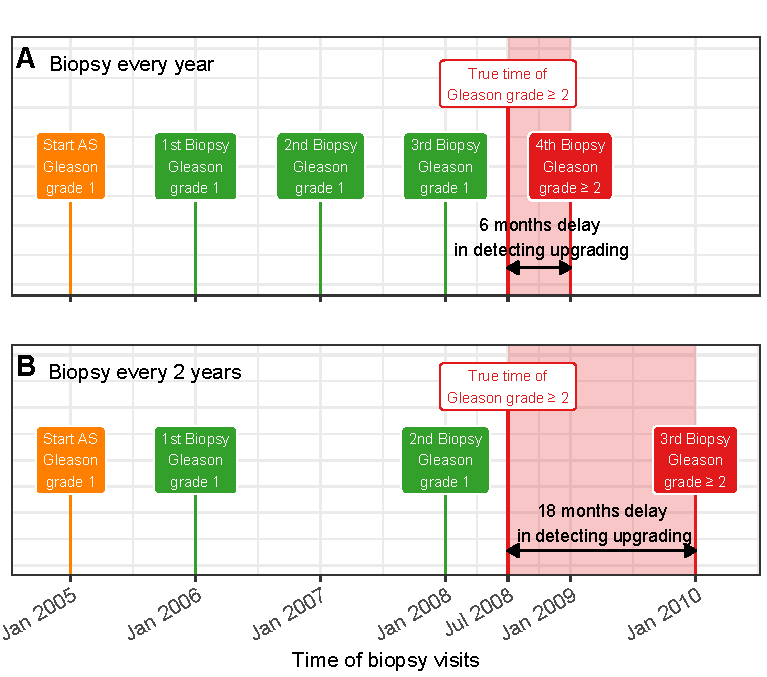
\includegraphics{contents/c5/images/c5_fig1.pdf}}
\caption{\textbf{Trade-off between the timing and number of biopsies (burden) and time delay in detecting Gleason upgrading (shorter is better):} The true time of Gleason upgrading (increase in Gleason grade group from group~1 to~2 or higher) for the patient in this figure is July 2008. When biopsies are scheduled annually (\textbf{Panel~A}), upgrading is detected in January 2009 with a time delay of six months, and a total of four biopsies are scheduled. When biopsies are scheduled biennially (\textbf{Panel~B}), upgrading is detected in January 2010 with a time delay of 18 months, and a total of three biopsies are scheduled. Since biopsies are conducted periodically, the time of upgrading is observed as an interval. For example, between Jan~2008--Jan~2009 in \textbf{Panel~A} and between Jan~2008--Jan~2010 in \textbf{Panel~B}. The phrase `Gleason grade group' is shortened to `Gleason grade' for brevity.}
\label{c5:fig:1}
\end{figure}

Except for the confirmatory biopsy at year one of AS~\citep{bokhorst2015compliance}, opinions and practice regarding the timing of remaining biopsies lack agreement~\citep{nieboer2018active}. Some AS programs utilize patients' observed PSA, DRE, previous biopsy Gleason grade, and lately, MRI results to decide biopsies~\citep{kasivisvanathan2020magnetic,bul2013active,nieboer2018active}. In contrast, others discourage schedules based on clinical data and MRI results~\citep{chesnut2019role,loeb2014heterogeneity}, and instead support periodical one-size-fits-all biopsy schedules. Furthermore, some suggest replacing frequent periodical schedules with infrequent ones (e.g., biennially)~\citep{inoue2018comparative,de2017estimating}. Each of these approaches has limitations. For example, one-size-fits-all schedules can lead to many unnecessary biopsies because of differences in baseline \emph{upgrading-risk} across cohorts~\citep{inoue2018comparative}. Whereas, since observed clinical data has measurement error (e.g., PSA fluctuations), a flaw of using it directly is that it may lead to poor decisions. Also, decisions based on clinical data typically rely only on the latest data point and ignore previous repeated measurements. A novel alternative that counters these drawbacks is first processing patient data via a statistical model, and subsequently using model predicted upgrading-risks to create \emph{personalized} biopsy schedules~\citep{nieboer2018active} (Figure~\ref{c5:fig:2}). While, upgrading-risk calculators are not new~\citep{coley2017prediction,ankerst2015precision,partin1993use,makarov2007updated}, not all are personalized either. Besides, they do not specify how risk predictions can be exploited to create a schedule.

\begin{figure}
\centerline{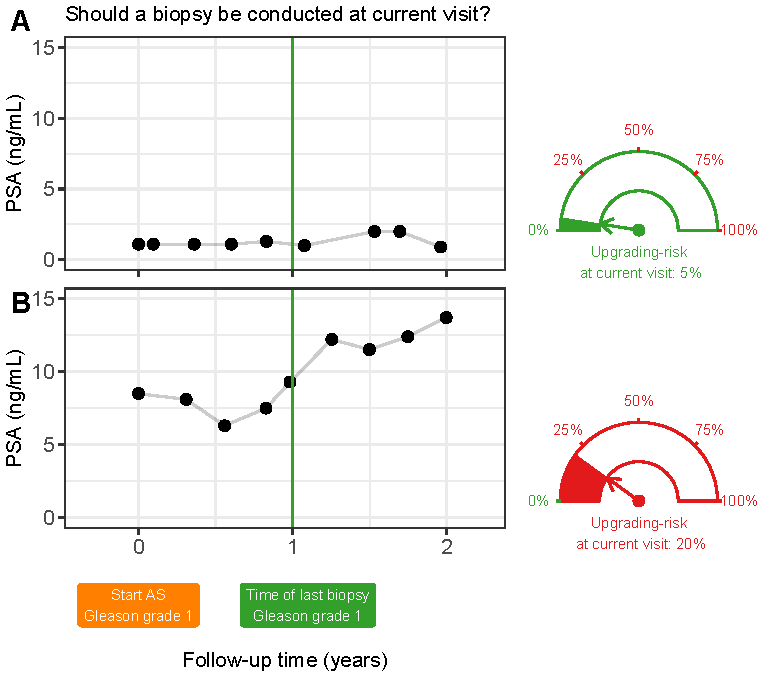
\includegraphics{contents/c5/images/c5_fig2.pdf}}
\caption{\textbf{Motivation for upgrading-risk based personalized biopsy decisions}: To utilize patients' complete longitudinal data and results from previous biopsies in making biopsy decisions. For this purpose, we first process data using a statistical model and then utilize the patient-specific predictions for risk of Gleason upgrading to schedule biopsies. For example, Patient~A (\textbf{Panel~A}) and B (\textbf{Panel~B}) had their latest biopsy at year one of follow-up (green vertical line). Patient~A's prostate-specific antigen (PSA) profile remained stable until his current visit at year two, whereas patient~B's profile has shown a rise. Consequently, patient~B's upgrading-risk at the current visit (year two) is higher than that of patient~A. This makes patient~B a more suitable candidate for biopsy than Patient~A. Risk estimates in this figure are only illustrative.}
\label{c5:fig:2}
\end{figure}

This work is motivated by the problem of scheduling biopsies in AS. We have two goals. First, we want to assist practitioners in using clinical data in biopsy decisions in a statistically sound manner. To this end, we plan to develop a robust, generalizable statistical model that provides reliable individual upgrading-risk in AS. Subsequently, we will employ these predictions to derive risk-based personalized biopsy schedules. Our second goal is to enable shared decision making of biopsy schedules. We intend to achieve this by allowing patients and doctors to compare the \emph{burden} and \emph{benefit} (Figure~\ref{c5:fig:1}) of opting for personalized schedules versus periodical schedules versus schedules based on clinical data. Specifically, we propose timing and number of planned biopsies (more/frequent are burdensome), and the expected time delay in detecting upgrading (shorter is beneficial) for any given schedule. While fulfilling our goals, we want to capture the maximum possible information from the available data. Hence, we will use all repeated measurements of patients, previous biopsy results, baseline characteristics, and keep our model flexible to accommodate future novel biomarkers. To fit this model, we will utilize data of the world's largest AS study, Prostate Cancer Research International Active Surveillance (PRIAS). To evaluate our model, we will externally validate it in the largest six AS cohorts from the Movember Foundation's Global Action Plan (GAP3) database~\citep{gap3_2018}. Last, we aim to implement the validated model and methodology in a web-application.
% !TEX root =  ../main_manuscript.tex 
\section{Patients and Methods}
\label{c5:sec:pat_methods}
\subsection{Study Cohort}
\label{subsec:cohort}
For developing a statistical model to predict upgrading-risk, we used the world's largest AS dataset, Prostate Cancer International Active Surveillance or PRIAS~\citep{bul2013active}, dated April 2019 (Table~\ref{table:prias_summary}). In PRIAS, biopsies were scheduled at year one, four, seven, ten, and additional yearly biopsies were scheduled when PSA doubling time was between zero and ten years. We selected all 7813~patients who had Gleason grade group~1 at inclusion in AS. Our primary event of interest is an increase in this Gleason grade group observed upon repeat biopsy, called \textit{upgrading} (1134~patients). Upgrading is a trigger for treatment advice in PRIAS. Some examples of treatment options in active surveillance are radical prostatectomy, brachytherapy, definitive radiation therapy, and other alternative local treatments such as cryosurgery, High Intensity Focused Ultrasound, and External Beam Radiation Therapy. Comprehensive details on treatment options and their side effects are available in EAU-ESTRO-SIOG guidelines on prostate cancer~\citep{mottet2017eau}. In PRIAS 2250 patients were provided treatment based on their PSA, the number of biopsy cores with cancer, or anxiety/other reasons. However, our reasons for focusing solely on upgrading are that upgrading is strongly associated with cancer-related outcomes, and other treatment triggers vary between cohorts~\citep{nieboer2018active}.

For externally validating our model's predictions, we selected the following largest (by the number of repeated measurements) six cohorts from Movember Foundation's GAP3 database~\citep{gap3_2018} version~3.1, covering nearly 73\% of the GAP3 patients: the University of Toronto AS (Toronto), Johns Hopkins AS (Hopkins), Memorial Sloan Kettering Cancer Center AS (MSKCC), King's College London AS (KCL), Michigan Urological Surgery Improvement Collaborative AS (MUSIC), and University of California San Francisco AS (UCSF, version~3.2). Only patients with a Gleason grade group~1 at the time of inclusion in these cohorts were selected. Summary statistics are presented in Section~\ref{c5:appendix:full_results}.

\begin{table}
\small
\centering
\caption{\textbf{Summary of the PRIAS dataset as of April 2019}. The primary event of interest is upgrading, that is, increase in Gleason grade group from group~1~\citep{epsteinGG2014} to 2 or higher. IQR:~interquartile range, PSA:~prostate-specific antigen. Study protocol URL: \url{https://www.prias-project.org}}
\label{table:prias_summary}
\begin{tabular}{lr}
\toprule
\textbf{Characteristic} & \textbf{Value}\\
\midrule
%Total centers & $> 100$\\
Total patients & 7813\\
Upgrading (primary event) & 1134\\
Treatment & 2250\\
Watchful waiting & 334\\
Loss to follow-up & 249\\
Death (unrelated to prostate cancer) & 95\\
Death (related to prostate cancer) & 2\\
\midrule
Median age at diagnosis (years) & 66 (IQR: 61--71)\\
Median maximum follow-up per patient (years) &  1.8 (IQR: 0.9--4.0)\\
Total PSA measurements & 67578\\
Median number of PSA measurements per patient &  6 (IQR: 4--12)\\
Median PSA value (ng/mL) & 5.7 (IQR: 4.1--7.7)\\
Total biopsies & 15686\\
Median number of biopsies per patient &  2 (IQR: 1--2)\\
\bottomrule
\end{tabular}
\end{table}

\paragraph{Choice of predictors:} In our model, we used all repeated PSA measurements, the timing of the previous biopsy and Gleason grade, and age at inclusion in AS. Other predictors such as prostate volume, MRI results can also be important. MRI is utilized already for targeting biopsies, but regarding its use in deciding the time of biopsies, there are arguments both for and against it~\citep{kasivisvanathan2020magnetic,chesnut2019role,schoots2015magnetic}. MRI is still a recent addition in most AS protocols. Consequently, repeated MRI data is very sparsely available in both PRIAS and GAP3 databases to make a stable prediction model. Prostate volume data is also sparsely available, especially in validation cohorts. Based on these reasons, we did not include them in our model. However, the model we propose next is extendable to include MRI and other novel biomarkers in the future.

% !TEX root =  ../main_manuscript.tex 
\subsection{Statistical Model}
Modeling an AS dataset such as PRIAS, posed certain challenges. First, PSA was measured longitudinally, and over follow-up time it did not always increase linearly. Consequently, we expect that PSA measurements of a patient are more similar to each other than of another patient. In other words, we need to accommodate the within-patient correlation for PSA. Second, PSA was available only until a patient observed upgrading. Thus, we also need to model the association between the Gleason grades and PSA profiles of a patient, and handle missing PSA measurements after a patient experienced upgrading. Third, since the PRIAS biopsy schedule uses PSA, a patient's observed time of upgrading was also dependent on their PSA. Thus, the effect of PSA on the upgrading-risk need to be adjusted for the effect of PSA on the biopsy schedule. Fourth, many patients obtained treatment and watchful waiting before observing upgrading. Since we considered events other than upgrading as censoring, the model needs to account for patients' reasons for treatment or watchful waiting (e.g., age, treatment based on observed data). A model that handles these challenges in a statistically sound manner is the joint model for time-to-event and longitudinal data~\citep{tomer2019,coley2017prediction,rizopoulos2012joint}.

Our joint model consisted of two sub-models. Namely, a linear mixed-effects sub-model~\citep{laird1982random} for longitudinally measured PSA (log-transformed), and a relative-risk sub-model (similar to the Cox model) for the interval-censored time of upgrading. Patient age was used in both sub-models. Results and timing of the previous negative biopsies were used only in the risk sub-model. To account for PSA fluctuations~\citep{nixon1997biological}, we assumed t-distributed PSA measurement errors. The correlation between PSA measurements of the same patient was established using patient-specific random-effects. We fitted a unique curve to the PSA measurements of each patient (Panel~A, Figure~\ref{c5:fig:3}). Subsequently, we calculated the mathematical derivative of the patient's fitted PSA profile~(\ref{c5:eq:rel_risk_model}), to obtain his follow-up time specific instantaneous PSA velocity (Panel~B, Figure~\ref{c5:fig:3}). This instantaneous velocity is a stronger predictor of upgrading than the widely used average PSA velocity~\citep{cooperberg2018refined}. We modeled the impact of PSA on upgrading-risk by employing fitted PSA value and instantaneous velocity as predictors in the risk sub-model (Panel~C, Figure~\ref{c5:fig:3}). We adjusted the effect of PSA on upgrading-risk for the PSA dependent PRIAS biopsy schedule by estimating parameters using a full likelihood method (proof in Chapter~\ref{c2:appendix:B}). This approach also accommodates watchful waiting and treatment protocols that are also based on patient data. Specifically, the parameters (Section~\ref{c5:appendix:model_specification}) of our two sub-models were estimated jointly under the Bayesian paradigm using the R package \textbf{JMbayes}~\citep{rizopoulosJMbayes}.

\begin{figure}
\centerline{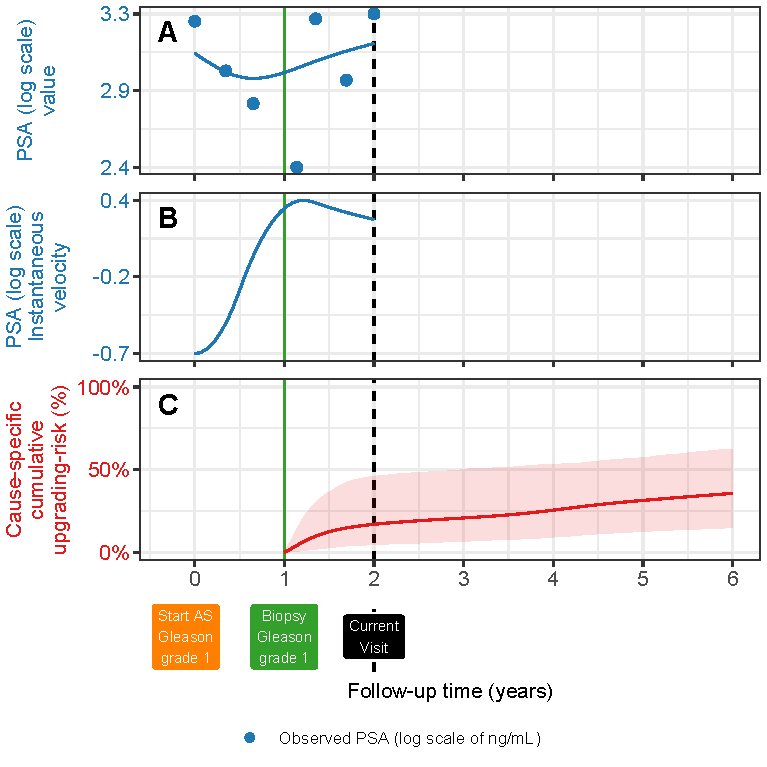
\includegraphics{contents/c5/images/c5_fig3.pdf}}
\caption{\textbf{Illustration of the joint model on a real PRIAS patient}. \textbf{Panel~A:} Observed PSA (blue dots) and fitted PSA (solid blue line), log-transformed from ng/mL. \textbf{Panel~B:} Estimated instantaneous velocity of PSA (log-transformed). \textbf{Panel~C}: Predicted cause-specific cumulative upgrading-risk (95\% credible interval shaded). Upgrading is defined as an increase in the Gleason grade group from group~1~\citep{epsteinGG2014} to 2 or higher. This upgrading-risk is calculated starting from the time of the latest negative biopsy (vertical green line at year one of follow-up). The joint model estimated it by combining the fitted PSA (log scale) value and instantaneous velocity, and time of the latest negative biopsy. Black dashed line at year two denotes the time of current visit.}
\label{c5:fig:3}
\end{figure}

\subsection{Risk Prediction and Model Validation}
Our model provides predictions for upgrading-risk over the entire future follow-up period of a patient (Panel~C, Figure~\ref{c5:fig:3}). However, we recommend using predictions only after year one. This is because most AS programs recommend a confirmatory biopsy at year one, especially to detect patients who may be misdiagnosed as low-grade at inclusion in AS. The model also automatically updates risk-predictions over follow-up as more patient data becomes available (Figure~\ref{c4:fig:2}). We validated our model internally in the PRIAS cohort, and externally in the largest six GAP3 database cohorts. We employed calibration plots~\citep{royston2013external,steyerberg2010assessing} and follow-up \textit{time-dependent} mean absolute risk prediction error or MAPE~\citep{rizopoulos2017dynamic} to graphically and quantitatively evaluate our model's risk prediction accuracy, respectively. We assessed our model's ability to discriminate between patients who experience/do not experience upgrading via the time-dependent area under the receiver operating characteristic curve or AUC~\citep{rizopoulos2017dynamic}. 

The aforementioned \textit{time-dependent} AUC and MAPE~\citep{rizopoulos2017dynamic} are temporal extensions of their standard versions~\citep{steyerberg2010assessing} in a longitudinal setting. Specifically, at every six months of follow-up, we calculated a unique AUC and MAPE for predicting upgrading-risk in the subsequent one year (Appendix~\ref{c5:appendix:validation}). For emulating a realistic situation, we calculated the AUC and MAPE at each follow-up using only the validation data available until that follow-up. Last, to resolve any potential model miscalibration in validation cohorts, we aimed to recalibrate our model's baseline hazard of upgrading (Appendix~\ref{c5:appendix:validation}), individually for each cohort.
% !TEX root =  ../main_manuscript.tex 
\section{Results}
The cause-specific cumulative upgrading-risk at year five of follow-up was 35\% in PRIAS and at most 50\% in validation cohorts (Panel~B, Figure~\ref{c5:fig:4}). In the fitted PRIAS model, the adjusted hazard ratio (aHR) of upgrading for an increase in patient age from 61 to 71 years (25-th to 75-th percentile) was 1.45~(95\%CI:~1.30--1.63). For an increase in fitted PSA value from 2.36 to 3.07 (25-th to 75-th percentile, log scale), the aHR was 0.99~(95\%CI:~0.89--1.11). The strongest predictor of upgrading-risk was instantaneous PSA velocity, with an increase from -0.09 to 0.31 (25-th to 75-th percentile), giving an aHR of 2.47~(95\%CI:~1.93--2.99). The aHR for PSA value and velocity was different in each GAP3 cohort (Table~\ref{c5:tab:PSA_survival_gap3}).

The time-dependent AUC, calibration plot, and time-dependent MAPE of our model are shown in Figure~\ref{c5:fig:4}, and Figure~\ref{c5:fig:auc_pe_recalib}. In all cohorts, time-dependent AUC was moderate (0.6 to 0.7) over the whole follow-up period. Time-dependent MAPE was moderate (0.1 to 0.2) in those cohorts where the impact of PSA on upgrading-risk was similar to PRIAS (e.g., Hopkins cohort, Table~\ref{c5:tab:PSA_survival_gap3}), and large (0.2 to 0.3) otherwise. Our model was miscalibrated for validation cohorts (Panel~B, Figure~\ref{c5:fig:4}), because cohorts had differences in inclusion criteria (e.g., PSA density) and follow-up protocols~\citep{gap3_2018} which were not accounted in our model. Consequently, the PRIAS based model's fitted baseline hazard did not correspond to the baseline hazard in validation cohorts. To solve this problem, we recalibrated the baseline hazard of upgrading in validation cohorts (Figure~\ref{c5:fig:calib_before_after}). We compared risk predictions from the recalibrated models, with predictions from separately fitted cohort-specific joint models (Figure~\ref{c5:fig:calib_in_small}). The difference in predictions was lowest in the Johns Hopkins cohort (impact of PSA on upgrading-risk similar to PRIAS). Comprehensive results are in Appendix~\ref{c5:appendix:full_results} and Appendix~\ref{c5:appendix:validation_res}.

\begin{figure}
\centerline{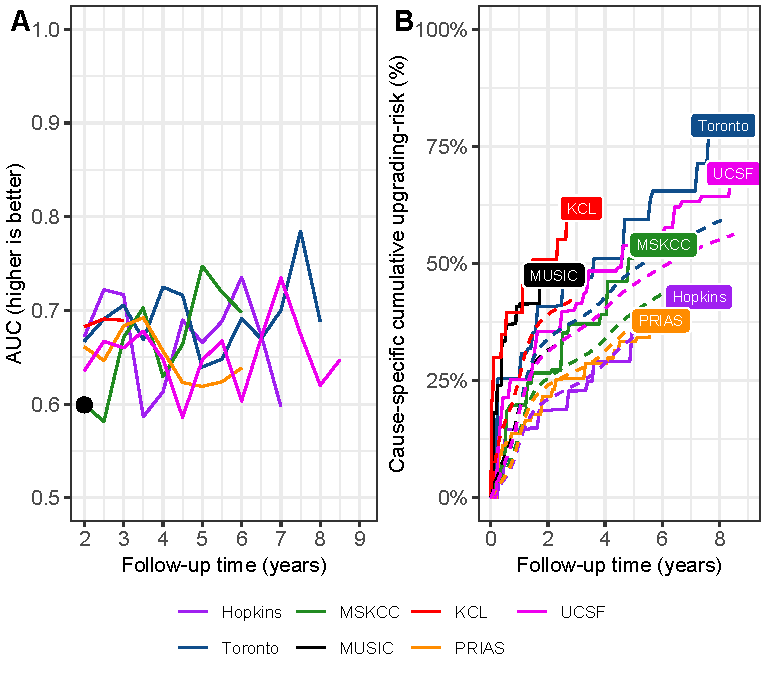
\includegraphics{contents/c5/images/c5_fig4.pdf}}
\caption{\textbf{Model Validation Results}. \textbf{Panel~A}: time-dependent area under the receiver operating characteristic curve or AUC (measure of discrimination). AUC at year one is not shown because we do not intend to replace the confirmatory biopsy at year one. \textbf{Panel~B}: calibration-at-large indicates model miscalibration. This is because solid lines depicting the non-parameteric estimate of the cause-specific cumulative upgrading-risk~\citep{turnbull1976empirical}, and dashed lines showing the average cause-specific cumulative upgrading-risk obtained using the joint model fitted to the PRIAS dataset, are not overlapping. Recalibrating the baseline hazard of upgrading resolved this issue (Figure~\ref{c5:fig:calib_before_after}). Full names of Cohorts are \textit{PRIAS}: Prostate Cancer International Active Surveillance, \textit{Toronto}: University of Toronto Active Surveillance, \textit{Hopkins}: Johns Hopkins Active Surveillance, \textit{MSKCC}: Memorial Sloan Kettering Cancer Center Active Surveillance, \textit{KCL}: King's College London Active Surveillance, \textit{MUSIC}: Michigan Urological Surgery Improvement Collaborative Active Surveillance, \textit{UCSF}: University of California San Francisco AS.}
\label{c5:fig:4}
\end{figure}

\subsection{Personalized Biopsy Schedules}
We employed the PRIAS based fitted model to create personalized biopsy schedules for real PRIAS patients. Particularly, first using the model and patient's observed data, we predicted his cumulative upgrading-risk (Figure~\ref{c5:fig:5}) on all of his future follow-up visits (biannually in PRIAS). Subsequently, we planned biopsies on those future visits where his conditional cumulative upgrading-risk was more than a certain threshold (see Chapter~\ref{c4:sec:schedule} for mathematical details). The choice of this threshold dictates the timing of biopsies in a risk-based personalized schedule. For example, personalized schedules based on 5\% and 10\% risk thresholds are shown in Figure~\ref{c5:fig:5}. 

To facilitate the choice of a risk-threshold, and for comparing the consequences of opting for a risk-based schedule versus any other schedule (e.g., annual, PRIAS), we predict expected time delay in detecting upgrading for following a schedule. We are able to predict this delay for any schedule. For example, in Panel~C of Figure~\ref{c5:fig:5}, the annual schedule has the least expected delay. In contrast, a personalized schedule based on a 10\% risk threshold has a slightly larger expected delay, but it also schedules much fewer biopsies. An important aspect of this delay is that it is personalized as well. That is, even if two different patients are prescribed the same biopsy schedule, their expected delays will be different. This is because delay is estimated using all available clinical data of the patient (Chapter~\ref{c4:subsec:exp_delay_estimation}). While the timing and the total number of planned biopsies denote the burden of a schedule, a shorter expected time delay in detecting upgrading can be a benefit. These two, along with other measures such as a patient's comorbidities, anxiety, etc., can help to make an informed biopsy decision.

\begin{figure}
\centerline{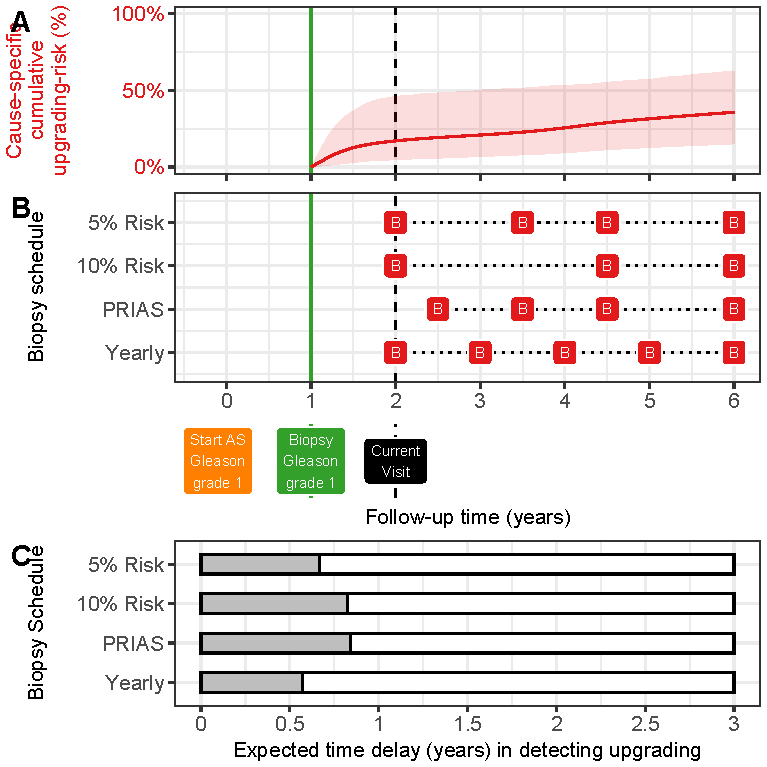
\includegraphics{contents/c5/images/c5_fig5.pdf}}
\caption{\textbf{Illustration of personalized and fixed schedules of biopsies for patient from Figure~\ref{c5:fig:3}}. \textbf{Panel~A:} Predicted cumulative upgrading-risk (95\% credible interval shaded). \textbf{Panel~B:} Different biopsy schedules with a red `B' indicating a future biopsy. Risk:~5\% and Risk:~10\% are personalized schedules in which a biopsy is planned whenever the conditional cause-specific cumulative upgrading-risk is above 5\% or 10\% risk, respectively. Green vertical line at year one is the time of the latest negative biopsy. Black dashed line at year two denotes the time of the current visit. \textbf{Panel~C:} Expected time delay in detecting upgrading (years) if patient progresses before year six. A compulsory biopsy was scheduled at year six (maximum biopsy scheduling time in PRIAS, Table~\ref{c5:tab:max_pred_time}) in all schedules for a meaningful comparison between them.}
\label{c5:fig:5}
\end{figure}

\subsection{Web-Application}
We implemented the PRIAS based model, recalibrated models for GAP3 cohorts, and personalized schedules in a user-friendly web-application \url{https://emcbiostatistics.shinyapps.io/prias_biopsy_recommender/}. This application works on both desktop and mobile devices. Patient data can be entered in Microsoft Excel format. The maximum follow-up time up to which predictions can be obtained depends on each cohort (Table~\ref{c5:tab:max_pred_time}). The web-application supports personalized, annual, and PRIAS schedules. For personalized schedules, users can control the choice of risk-threshold. The web-application also compares the resulting risk-based schedule's timing of biopsies, and expected time delay in detecting upgrading, with annual and PRIAS schedules, to enable sharing biopsy decision making.
% !TEX root =  ../main_manuscript.tex 
\section{Discussion}
We successfully developed and externally validated a statistical model for predicting upgrading-risk~\citep{bruinsma2017expert} in prostate cancer AS, and providing risk-based personalized biopsy decisions. Our work has four novel features over earlier risk calculators~\citep{coley2017prediction,ankerst2015precision}. First, our model was fitted to the world's largest AS dataset PRIAS and externally validated in the largest six cohorts of the Movember Foundation's GAP3 database~\citep{gap3_2018}. Second, the model predicts a patient's current and future upgrading-risk in a personalized manner. Third, using the predicted risks, we created personalized biopsy schedules. We also calculated the expected time delay in detecting upgrading (less is beneficial) for following any schedule. Thus, patients/doctors can compare schedules before making a choice. Fourth, we implemented our methodology in a user-friendly web-application (\url{https://emcbiostatistics.shinyapps.io/prias_biopsy_recommender/}) for both PRIAS and validated cohorts.

Our model and methods can be useful for numerous patients from PRIAS and the validated GAP3 cohorts (nearly 73\% of all GAP3 patients). The model utilizes all repeated PSA measurements, results of previous biopsies, and baseline characteristics of a patient. We could not include MRI and PSA density because of sparsely available data in both PRIAS and GAP3 databases. But, our model is extendable to include them in the near future. The current discrimination ability of our model, exhibited by the \textit{time-dependent} AUC, was between 0.6 and 0.7 over-follow. While this is moderate, it is also so because unlike the standard AUC~\citep{steyerberg2010assessing} the time-dependent AUC is more conservative as it utilizes only the validation data available until the time at which it is calculated. The same holds for the time-dependent MAPE (mean absolute prediction error). Although, MAPE varied much more between cohorts than AUC. In cohorts where the effect size for the impact of PSA value and velocity on upgrading-risk was similar to that for PRIAS (e.g., Hopkins cohort), MAPE was moderate. Otherwise, MAPE was large (e.g., KCL and MUSIC cohorts). We required recalibration of our model's baseline hazard of upgrading for all validation cohorts.

The clinical implications of our work are as follows. First, the cause-specific cumulative upgrading-risk at year five of follow-up was at most 50\% in all cohorts (Panel~B, Figure~\ref{c5:fig:4}). That is, many patients may not require some of the biopsies planned in the first five years of AS. Given the non-compliance and burden of frequent biopsies~\citep{bokhorst2015compliance}, the availability of our methodology as a web-application may encourage patients/doctors to consider upgrading-risk based personalized schedules instead. An additional advantage of personalized schedules is that they update as more patient data becomes available over follow-up. Despite the moderate predictive performance, we expect the overall impact of our model to be positive. There are two reasons for this. First, the risk of adverse outcomes because of the use of personalized schedules is quite low because of the low rate of metastases and prostate cancer specific mortality in AS patients (Table~\ref{table:prias_summary}). Second, studies~\citep{carvalho2017,inoue2018comparative} have suggested that after the confirmatory biopsy at year one of follow-up, biopsies may be done as infrequently as every two to three years, with limited adverse consequences. In other words, longer delays in detecting upgrading may be acceptable after the first negative biopsy. To evaluate the potential harm of personalized schedules, we compared them with fixed schedules in a realistic and extensive simulation study~\citep{tomer2019personalized}. We concluded that personalized schedules plan, on average, six fewer biopsies compared to annual schedule and two fewer biopsies than the PRIAS schedule in slow/non-progressing AS patients, while maintaining almost the same time delay in detecting upgrading as PRIAS schedule. Personalized schedules with different risk thresholds indeed have different performances across cohorts. Thus, to assist patients/doctors in choosing between fixed schedules and personalized schedules based on different risk thresholds, the web-application provides a patient-specific estimate of the expected time delay in detecting upgrading, for both personalized and fixed schedules. We hope that access to these estimates will objectively address patient apprehensions regarding adverse outcomes in AS. Last, we note that our web-application should only be used to decide biopsies after the compulsory confirmatory biopsy at year one of follow-up.

This work has certain limitations. Predictions for upgrading-risk and personalized schedules are available only for a currently limited, cohort-specific, follow-up period (Table~\ref{c5:tab:max_pred_time}). This problem can be mitigated by refitting the model with new follow-up data in the future. Recently, some cohorts started utilizing MRI to explore the possibility of targeting visible lesions by biopsy. Presently, the GAP3 database has limited PSA density and MRI follow-up data available. Since PSA density is used as an entry criterion in some active surveillance studies, including it as a predictor can improve the model. Although, the current model can be extended to include both MRI and PSA density data as predictors when they become available in future. We scheduled biopsies using cause-specific cumulative upgrading-risk, which ignores competing events such as treatment based on the number of positive biopsy cores. Employing a competing-risk model may lead to improved personalized schedules. Upgrading is susceptible to inter-observer variation too. Models which account for this variation~\citep{coley2017prediction,balasubramanian2003estimation} will be interesting to investigate further. Even with an enhanced risk prediction model, the methodology for personalized scheduling and calculation of expected time delay (Chapter~\ref{c4:subsec:exp_delay_estimation}) need not change. Last, our web-application only allows uploading patient data in Microsoft Excel format. Connecting it with patient databases can increase usability.
% !TEX root =  ../main_manuscript.tex 
\section{Conclusions}
We successfully developed a statistical model and methodology for predicting upgrading-risk, and providing risk-based personalized biopsy decisions, in prostate cancer AS. We externally validated our model, covering nearly 73\% patients from the Movember Foundations' GAP3 database. The model made available via a user-friendly web-application (\url{https://emcbiostatistics.shinyapps.io/prias_biopsy_recommender/}) enables shared decision making of biopsy schedules by comparing fixed and personalized schedules on total biopsies and expected time delay in detecting upgrading. Novel biomarkers and MRI data can be added as predictors in the model to improve predictions in the future. Recalibration of baseline upgrading-risk is advised for cohorts not validated in this work.

\paragraph{Acknowledgements}
We thank Jozien Helleman from the Department of Urology, Erasmus University Medical Center, for coordinating the project. The first and last authors would like to acknowledge support by Nederlandse Organisatie voor Wetenschappelijk Onderzoek (the national research council of the Netherlands) VIDI grant nr. 016.146.301, and Erasmus University Medical Center funding. Part of this work was carried out on the Dutch national e-infrastructure with the support of SURF Cooperative. The authors also thank the Erasmus University Medical Center's Cancer Computational Biology Center for giving access to their IT-infrastructure and software that was used for the computations and data analysis in this study. The PRIAS website is funded by the Prostate Cancer Research Foundation, Rotterdam (SWOP). We would like to thank the PRIAS consortium for enabling this research project. 

This work was supported by the Movember Foundation. The funder did not play any role in the study design, collection, analysis or interpretation of data, or in the drafting of this paper.

\paragraph{Conflicts of Interest}
The authors do not report any conflict of interest, and have nothing to disclose.
\section*{Members of The Movember Foundation’s Global Action Plan Prostate Cancer Active Surveillance (GAP3) consortium}

\emph{Principle Investigators:} Bruce Trock (Johns Hopkins University, The James Buchanan Brady Urological Institute, Baltimore, USA), Behfar Ehdaie (Memorial Sloan Kettering Cancer Center, New York, USA), Peter Carroll (University of California San Francisco, San Francisco, USA), Christopher Filson (Emory University School of Medicine, Winship Cancer Institute, Atlanta, USA), Jeri Kim / Christopher Logothetis (MD Anderson Cancer Centre, Houston, USA), Todd Morgan (University of Michigan and Michigan Urological Surgery Improvement Collaborative (MUSIC), Michigan, USA), Laurence Klotz (University of Toronto, Sunnybrook Health Sciences Centre, Toronto, Ontario, Canada), Tom Pickles (University of British Columbia, BC Cancer Agency, Vancouver, Canada), Eric Hyndman (University of Calgary, Southern Alberta Institute of Urology, Calgary, Canada), Caroline Moore (University College London \& University College London Hospital Trust, London, UK), Vincent Gnanapragasam (University of Cambridge \& Cambridge University Hospitals NHS Foundation Trust, Cambridge, UK), Mieke Van Hemelrijck (King's College London, London, UK \& Guy’s and St Thomas’ NHS Foundation Trust, London, UK), Prokar Dasgupta (Guy’s and St Thomas’ NHS Foundation Trust, London, UK), Chris Bangma (Erasmus Medical Center, Rotterdam, The Netherlands/ representative of Prostate cancer Research International Active Surveillance (PRIAS) consortium), Monique Roobol (Erasmus Medical Center, Rotterdam, The Netherlands/ representative of Prostate cancer Research International Active Surveillance (PRIAS) consortium), The PRIAS study group, Arnauld Villers (Lille University Hospital Center, Lille, France), Antti Rannikko (Helsinki University and Helsinki University Hospital, Helsinki, Finland), Riccardo Valdagni (Department of Oncology and Hemato-oncology, Università degli Studi di Milano, Radiation Oncology 1 and Prostate Cancer Program, Fondazione IRCCS Istituto Nazionale dei Tumori, Milan, Italy), Antoinette Perry (University College Dublin, Dublin, Ireland), Jonas Hugosson (Sahlgrenska University Hospital, Göteborg, Sweden), Jose Rubio-Briones (Instituto Valenciano de Oncología, Valencia, Spain), Anders Bjartell (Skåne University Hospital, Malmö, Sweden), Lukas Hefermehl (Kantonsspital Baden, Baden, Switzerland), Lee Lui Shiong (Singapore General Hospital, Singapore, Singapore), Mark Frydenberg (Monash Health; Monash University, Melbourne, Australia), Yoshiyuki Kakehi / Mikio Sugimoto (Kagawa University Faculty of Medicine, Kagawa, Japan), Byung Ha Chung (Gangnam Severance Hospital, Yonsei University Health System, Seoul, Republic of Korea)

\emph{Pathologist:} Theo van der Kwast (Princess Margaret Cancer Centre, Toronto, Canada). 
Technology Research Partners: Henk Obbink (Royal Philips, Eindhoven, the Netherlands), Wim van der Linden (Royal Philips, Eindhoven, the Netherlands), Tim Hulsen (Royal Philips, Eindhoven, the Netherlands), Cees de Jonge (Royal Philips, Eindhoven, the Netherlands).

\emph{Advisory Regional statisticians:} Mike Kattan (Cleveland Clinic, Cleveland, Ohio, USA), Ji Xinge (Cleveland Clinic, Cleveland, Ohio, USA), Kenneth Muir (University of Manchester, Manchester, UK), Artitaya Lophatananon (University of Manchester, Manchester, UK), Michael Fahey (Epworth HealthCare, Melbourne, Australia), Ewout Steyerberg (Erasmus Medical Center, Rotterdam, The Netherlands), Daan Nieboer (Erasmus Medical Center, Rotterdam, The Netherlands); Liying Zhang (University of Toronto, Sunnybrook Health Sciences Centre, Toronto, Ontario, Canada)

\emph{Executive Regional statisticians:} Ewout Steyerberg (Erasmus Medical Center, Rotterdam, The Netherlands), Daan Nieboer (Erasmus Medical Center, Rotterdam, The Netherlands); Kerri Beckmann (King's College London, London, UK \& Guy’s and St Thomas’ NHS Foundation Trust, London, UK), Brian Denton (University of Michigan, Michigan, USA), Andrew Hayen (University of Technology Sydney, Australia), Paul Boutros (Ontario Institute of Cancer Research, Toronto, Ontario, Canada).

\emph{Clinical Research Partners’ IT Experts:} Wei Guo (Johns Hopkins University, The James Buchanan Brady Urological Institute, Baltimore, USA), Nicole Benfante (Memorial Sloan Kettering Cancer Center, New York, USA), Janet Cowan (University of California San Francisco, San Francisco, USA), Dattatraya Patil (Emory University School of Medicine, Winship Cancer Institute, Atlanta, USA), Emily Tolosa (MD Anderson Cancer Centre, Houston, Texas, USA), Tae-Kyung Kim (University of Michigan and Michigan Urological Surgery Improvement Collaborative, Ann Arbor, Michigan, USA), Alexandre Mamedov (University of Toronto, Sunnybrook Health Sciences Centre, Toronto, Ontario, Canada), Vincent LaPointe (University of British Columbia, BC Cancer Agency, Vancouver, Canada), Trafford Crump (University of Calgary, Southern Alberta Institute of Urology, Calgary, Canada), Vasilis Stavrinides (University College London \& University College London Hospital Trust, London, UK), Jenna Kimberly-Duffell (University of Cambridge \& Cambridge University Hospitals NHS Foundation Trust, Cambridge, UK), Aida Santaolalla (King's College London, London, UK \& Guy’s and St Thomas’ NHS Foundation Trust, London, UK), Daan Nieboer (Erasmus Medical Center, Rotterdam, The Netherlands), Jonathan Olivier (Lille University Hospital Center, Lille, France), Tiziana Rancati (Fondazione IRCCS Istituto Nazionale dei Tumori di Milano, Milan, Italy), Helén Ahlgren (Sahlgrenska University Hospital, Göteborg, Sweden), Juanma Mascarós (Instituto Valenciano de Oncología, Valencia, Spain), Annica Löfgren (Skåne University Hospital, Malmö, Sweden), Kurt Lehmann (Kantonsspital Baden, Baden, Switzerland), Catherine Han Lin (Monash University and Epworth HealthCare, Melbourne, Australia), Hiromi Hirama (Kagawa University, Kagawa, Japan), Kwang Suk Lee (Yonsei University College of Medicine, Gangnam Severance Hospital, Seoul, Korea). 

\emph{Research Advisory Committee:} Guido Jenster (Erasmus MC, Rotterdam, the Netherlands), Anssi Auvinen (University of Tampere, Tampere, Finland), Anders Bjartell (Skåne University Hospital, Malmö, Sweden), Masoom Haider (University of Toronto, Toronto, Canada), Kees van Bochove (The Hyve B.V. Utrecht, Utrecht, the Netherlands), Ballentine Carter (Johns Hopkins University, Baltimore, USA – until 2018). 

\emph{Management team:} Sam Gledhill (Movember Foundation, Melbourne, Australia), Mark Buzza / Michelle Kouspou (Movember Foundation, Melbourne, Australia), Chris Bangma (Erasmus Medical Center, Rotterdam, The Netherlands), Monique Roobol (Erasmus Medical Center, Rotterdam, The Netherlands), Sophie Bruinsma / Jozien Helleman (Erasmus Medical Center, Rotterdam, The Netherlands).

\section*{Appendix}
\begin{subappendices}

\section{Model Specification}
\label{c5:appendix:model_specification}
Let $T_i^*$ denote the true time of upgrading (increase in biopsy Gleason grade group from~1 to 2 or higher) for the ${i\mbox{-th}}$ patient included in PRIAS. Since biopsies are conducted periodically, $T_i^*$ is observed with interval censoring ${l_i < T_i^* \leq r_i}$. When upgrading is observed for the patient at his latest biopsy time $r_i$, then $l_i$ denotes the time of the second latest biopsy. Otherwise, $l_i$ denotes the time of the latest biopsy and ${r_i=\infty}$. Let $\boldsymbol{y}_{i}$ denote his observed PSA longitudinal measurements. The observed data of all $n$ patients is denoted by ${\mathcal{A}_n = \{l_i, r_i, \boldsymbol{y}_{i}; i = 1, \ldots, n\}}$.

In our joint model, the patient-specific PSA measurements over time are modeled using a linear mixed effects sub-model. It is given by (see Panel~A, Figure~\ref{c5:fig:3}):
\begin{equation}
\label{c5:eq:long_model_psa}
\begin{split}
    \log_2 \big\{y_{i}(t) + 1\big\} &= m_{i}(t) + \varepsilon_{i}(t),\\
    m_{i}(t) &= \beta_{0} + b_{0i} + \sum_{k=1}^4 (\beta_{k} + b_{ki})  B_k\Big(\frac{t-2}{2},\frac{\mathcal{K}-2}{2}\Big)\\
    & \quad + \beta_{5} \mbox{age}_i,
    \end{split}
\end{equation}
where, $m_{i}(t)$ denotes the measurement error free value of $\log_2 (\mbox{PSA} + 1)$ transformed \citep{pearson1994mixed,lin2000latent} measurements at time $t$. We model it non-linearly over time using B-splines \citep{de1978practical}. To this end, our B-spline basis function ${B_k\{(t-2)/2,(\mathcal{K}-2)/2\}}$ has three internal knots at $\mathcal{K} = \{0.5, 1.3, 3\}$ years, which are the three quartiles of the observed follow-up times. The boundary knots of the spline are at 0 and 6.3 years (95-th percentile of the observed follow-up times). We mean centered (mean 2 years) and standardized (standard deviation 2 years) the follow-up time $t$ and the knots of the B-spline $\mathcal{K}$ during parameter estimation for better convergence. The fixed effect parameters are denoted by ${\{\beta_{0},\ldots,\beta_{5}\}}$, and ${\{b_{0i}, \ldots, b_{4i}\}}$ are the patient specific random effects. The random effects follow a multivariate normal distribution with mean zero and variance-covariance matrix $\boldsymbol{W}$. The error $\varepsilon_{i}(t)$ is assumed to be t-distributed with three degrees of freedom and scale $\sigma$, and is independent of the random effects. 

To model the impact of PSA measurements on the risk of upgrading, our joint model uses a relative risk sub-model. More specifically, the hazard of upgrading denoted as $h_i(t)$, and the cumulative-risk of upgrading denoted as $R_i(t)$, at a time $t$ are (see Panel~C, Figure~\ref{c5:fig:3}):
\begin{equation}
\label{c5:eq:rel_risk_model}
\begin{split}
    h_i(t) &= h_0(t) \exp\Big(\gamma \mbox{age}_i +\alpha_{1} m_{i}(t) + \alpha_{2} \frac{\mathrm{d}m_{i}(t)}{\mathrm{d}{t}}\Big),\\
    R_i(t) &= \exp\Big\{-\int_0^{t} h_i(s)\mathrm{d}{s}\Big\},
    \end{split}
\end{equation}
where, $\gamma$ is the parameter for the effect of age. The impact of PSA on the hazard of upgrading is modeled in two ways, namely the impact of the error free underlying PSA value $m_{i}(t)$ (see Panel~A, Figure~\ref{c5:fig:3}), and the impact of the underlying PSA velocity $\mathrm{d}m_{i}(t)/\mathrm{d}{t}$ (see Panel~B, Figure~\ref{c5:fig:3}). The corresponding parameters are $\alpha_{1}$ and $\alpha_{2}$, respectively. Lastly, $h_0(t)$ is the baseline hazard at time t, and is modeled flexibly using P-splines \citep{eilers1996flexible}. More specifically:
\begin{equation*}
\log{h_0(t)} = \gamma_{h_0,0} + \sum_{q=1}^Q \gamma_{h_0,q} B_q(t, \boldsymbol{v}),
\end{equation*}
where $B_q(t, \boldsymbol{v})$ denotes the $q$-th basis function of a B-spline with knots $\boldsymbol{v} = v_1, \ldots, v_Q$ and vector of spline coefficients $\gamma_{h_0}$. To avoid choosing the number and position of knots in the spline, a relatively high number of knots (e.g., 15 to 20) are chosen and the corresponding B-spline regression coefficients $\gamma_{h_0}$ are penalized using a differences penalty \citep{eilers1996flexible}.

\section{Full Results}
\label{c5:appendix:full_results}
Characteristics of the six validation cohorts from the GAP3 database~\citep{gap3_2018} are shown in Table~\ref{c5:tab:gap3_summary_1}, Table~\ref{c5:tab:gap3_summary_2}, and Table~\ref{c5:tab:gap3_summary_3}. The cause-specific cumulative upgrading-risk in these cohorts is shown in Figure~\ref{c5:fig:app1}.

\begin{figure}
\centerline{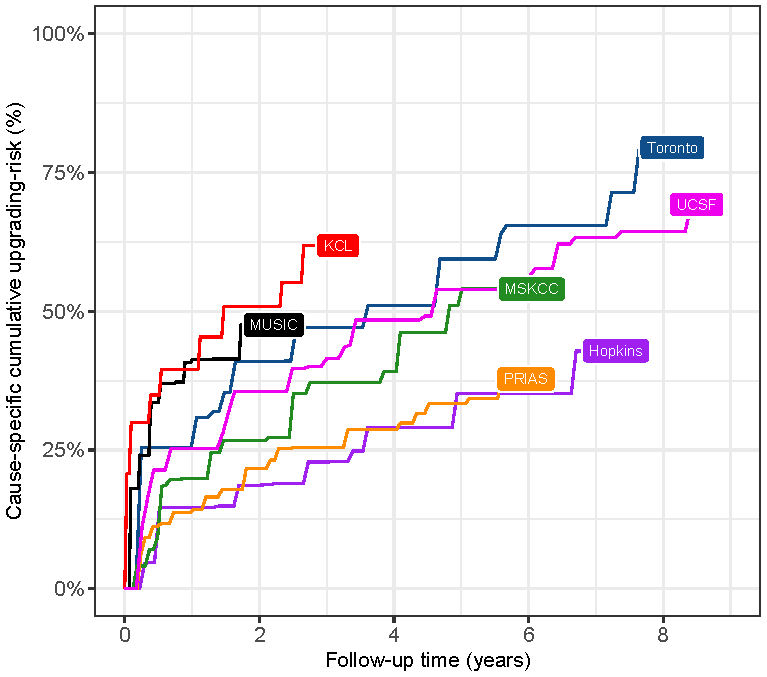
\includegraphics{contents/c5/images/c5_fig_app1.pdf}}
\caption{\textbf{Nonparametric estimate \citep{turnbull1976empirical} of the cause-specific cumulative upgrading-risk} in the world's largest AS cohort PRIAS, and largest six AS cohorts from the GAP3 database \citep{gap3_2018}. Abbreviations are \textit{Hopkins}: Johns Hopkins Active Surveillance, \textit{PRIAS}: Prostate Cancer International Active Surveillance, \textit{Toronto}: University of Toronto Active Surveillance, \textit{MSKCC}: Memorial Sloan Kettering Cancer Center Active Surveillance, \textit{KCL}: King's College London Active Surveillance, \textit{MUSIC}: Michigan Urological Surgery Improvement Collaborative AS, \textit{UCSF}: University of California San Francisco Active Surveillance.}
\label{c5:fig:app1}
\end{figure}

\begin{table}
\small
\centering
\caption{\textbf{Summary of the Hopkins and Toronto validation cohorts from the GAP3 database~\citep{gap3_2018}}. The primary event of interest is upgrading, that is, increase in Gleason grade group from group~1 to 2 or higher. \#PSA: number of PSA, \#biopsies: number of biopsies, IQR:~interquartile range, PSA:~prostate-specific antigen. Full names of cohorts are \textit{Hopkins}: Johns Hopkins Active Surveillance, \textit{Toronto}: University of Toronto Active Surveillance}
\label{c5:tab:gap3_summary_1}
\begin{tabular}{p{5cm}rr}
\hline
\textbf{Characteristic} & \textbf{Hopkins} & \textbf{Toronto}\\
\hline
Total patients & 1392 & 1046\\
Upgrading (primary event) & 260 & 359\\
\hline
Median age (years) & 62 (IQR: 66--69) & 67 (IQR: 60--72)\\
Median maximum follow-up per patient (years) &  3 (IQR: 1.3--5.8) & 4.5 (IQR: 1.9--8.4)\\
Total PSA measurements & 11126 & 13984\\
Median \#PSA per patient &  6 (IQR: 4--11) & 12 (IQR: 7--19)\\
Median PSA (ng/mL) & 4.7 (IQR: 2.9--6.7) & 6 (IQR: 3.7--9.0)\\
Total biopsies & 1926 & 909\\
Median \#biopsies per patient &  1 (IQR: 1--2) &  1 (IQR: 1--2)\\
\hline
\end{tabular}
\end{table}

\begin{table}
\small
\centering
\caption{\textbf{Summary of the MSKCC and UCSF validation cohorts from the GAP3 database~\citep{gap3_2018}}. The primary event of interest is upgrading, that is, increase in Gleason grade group from group~1 to 2 or higher. \#PSA: number of PSA, \#biopsies: number of biopsies, IQR:~interquartile range, PSA:~prostate-specific antigen. Full names of cohorts are \textit{MSKCC}: Memorial Sloan Kettering Cancer Center Active Surveillance, \textit{UCSF}: University of California San Francisco Active Surveillance.}
\label{c5:tab:gap3_summary_2}
\begin{tabular}{p{5cm}rr}
\hline
\textbf{Characteristic} & \textbf{MSKCC} & \textbf{UCSF}\\
\hline
Total patients & 894 & 1397 \\
Upgrading (primary event) & 242 & 547\\
\hline
Median age (years) & 63 (IQR: 57--68) & 63 (IQR: 57--68)\\
Median maximum follow-up per patient (years) & 5.3 (IQR: 1.8--8.3) & 3.6 (IQR: 1.5--7.2)\\
Total PSA measurements & 10704 & 16093\\
Median \#PSA per patient & 11 (IQR: 5--17) & 8 (IQR: 4--16)\\
Median PSA (ng/mL) & 4.7 (IQR: 2.8--7.1) & 5.0 (IQR: 3.4--7.2)\\
Total biopsies & 1102 & 3512\\
Median \#biopsies per patient & 1 (IQR: 1--2) & 2 (IQR: 2--3)\\
\hline
\end{tabular}
\end{table}

\begin{table}
\small
\centering
\caption{\textbf{Summary of the MUSIC and KCL validation cohorts from the GAP3 database~\citep{gap3_2018}}. The primary event of interest is upgrading, that is, increase in Gleason grade group from group~1 to 2 or higher. \#PSA: number of PSA, \#biopsies: number of biopsies, IQR:~interquartile range, PSA:~prostate-specific antigen. Full names of cohorts are \textit{KCL}: King's College London Active Surveillance, \textit{MUSIC}: Michigan Urological Surgery Improvement Collaborative AS.}
\label{c5:tab:gap3_summary_3}
\begin{tabular}{p{5cm}rr}
\hline
\textbf{Characteristic} & \textbf{MUSIC} & \textbf{KCL}\\
\hline
Total patients & 2743 & 616\\
Upgrading (primary event) & 385 & 198\\
\hline
Median age (years) & 65 (IQR: 60--71) & 63 (IQR: 58--68)\\
Median maximum follow-up per patient (years) & 1.2 (IQR: 0.6--2.2) & 2.4 (IQR: 1.3--3.8)\\
Total PSA measurements & 12087 & 2987\\
Median \#PSA per patient & 4 (IQR: 2--6) & 4 (IQR: 2--6)\\
Median PSA (ng/mL) & 5.1 (IQR: 3.4--7.1) & 6 (IQR: 4--9)\\
Total biopsies & 1032 & 484\\
Median \#biopsies per patient & 1 (IQR: 1--1) & 1 (IQR: 1--1)\\
\hline
\end{tabular}
\end{table}

For the relative risk sub-model, the parameter estimates in Table~\ref{c5:tab:PSA_survival} show that ${\log_2 (\mbox{PSA} + 1)}$ velocity and age of the patient were significantly associated with the hazard of upgrading.

\begin{table}
\small
\centering
\caption{\textbf{Parameters of the relative risk sub-model}: Estimated mean and 95\% credible interval for the parameters of the relative-risk sub-model.}
\label{c5:tab:PSA_survival}
\begin{tabular}{lrrrrr}
\hline
Variable                      & Mean   & Std. Dev & 2.5\%  & 97.5\%                 & P              \\
\hline
Age                      & 0.037    & 0.006 & 0.025  & 0.049  & \textless0.001 \\
Fitted $\log_2 (\mbox{PSA} + 1)$ value            & -0.012   & 0.076 & -0.164 & 0.135  & 0.856 \\
Fitted $\log_2 (\mbox{PSA} + 1)$ velocity             & 2.266    & 0.299 & 1.613  & 2.767  & \textless0.001   \\
\hline
\end{tabular}
\end{table}

It is important to note that since age, and ${\log_2 (\mbox{PSA} + 1)}$ value and velocity are all measured on different scales, a comparison between the corresponding parameter estimates is not easy. To this end, in Table \ref{c5:tab:PSA_survival_easy}, we present the hazard ratio of upgrading, for an increase in the aforementioned variables from their 25-th to the 75-th percentile. For example, an increase in fitted $\log_2 (\mbox{PSA} + 1)$ velocity from -0.085 to 0.308 (fitted 25-th and 75-th percentiles) corresponds to a hazard ratio of 2.433. The interpretation of the rest is similar.

\begin{table}
\small
\centering
\caption{\textbf{Hazard ratio and 95\% credible interval (CI) for upgrading}: Variables are on different scale and hence we compare an increase in the variables of relative risk sub-model from their 25-th percentile ($\mbox{P}_{25}$) to their 75-th percentile ($\mbox{P}_{75}$). Except for age, quartiles for all other variables are based on their fitted values obtained from the joint model fitted to the PRIAS dataset.}
\label{c5:tab:PSA_survival_easy}
\begin{tabular}{lrrr}
\hline
Variable                      & $\mbox{P}_{25}$   & $\mbox{P}_{75}$ & Hazard ratio [95\% CI] \\
\hline
Age & 61 & 71 & 1.455 [1.285, 1.631] \\
Fitted $\log_2 (\mbox{PSA} + 1)$ value & 2.360 & 3.078 & 0.991 [0.889, 1.102] \\
Fitted $\log_2 (\mbox{PSA} + 1)$ velocity & -0.085 & 0.308 & 2.433 [1.883, 2.962] \\
\hline
\end{tabular}
\end{table}

\begin{table}
\small
\centering
\caption{\textbf{Parameters of the relative risk sub-model in validation cohorts}. We fitted separate joint models for each of the six GAP3 validation cohorts as well. The specification of these joint models was same as that of the model for PRIAS. Two important predictors in the relative-risk sub-model, namely, the $\log_2 (\mbox{PSA} + 1)$ value and velocity have different impact on upgrading-risk across the cohorts. Table shows the mean estimate of these parameters with 95\% credible interval in brackets. Strongest average effect of $\log_2 (\mbox{PSA} + 1)$ velocity is in PRIAS cohort, whereas the weakest is in MUSIC cohort. The strongest average effect of $\log_2 (\mbox{PSA} + 1)$ value is in the Toronto cohort whereas the weakest is in PRIAS cohort. Full names of cohorts are \textit{Hopkins}: Johns Hopkins Active Surveillance, \textit{PRIAS}: Prostate Cancer International Active Surveillance, \textit{Toronto}: University of Toronto Active Surveillance, \textit{MSKCC}: Memorial Sloan Kettering Cancer Center Active Surveillance, \textit{KCL}: King's College London Active Surveillance, \textit{MUSIC}: Michigan Urological Surgery Improvement Collaborative AS, \textit{UCSF}: University of California San Francisco Active Surveillance.}
\label{c5:tab:PSA_survival_gap3}
\begin{tabular}{lrr}
\hline
Cohort & Fitted $\log_2 (\mbox{PSA} + 1)$ value & Fitted $\log_2 (\mbox{PSA} + 1)$ velocity\\
\hline
PRIAS & -0.012 [-0.164, 0.135] & 2.266 [ 1.613, 2.767]\\
Hopkins & 0.061 [-0.323, 0.329] & 1.839 [ 0.761, 4.378]\\
MSKCC & 0.336 [ 0.081, 0.583] & 1.122 [ 0.421, 1.980]\\
Toronto & 0.572 [ 0.347, 0.794] & 0.943 [ 0.464, 1.554]\\
UCSF & 0.498 [ 0.326, 0.673] & 0.812 [ 0.280, 1.383]\\
MUSIC & 0.441 [ 0.092, 0.767] & 0.029 [-0.552, 0.512]\\
KCL &  0.194 [-0.104, 0.540] & 0.840 [-0.087, 1.665]\\
\hline
\end{tabular}
\end{table}

\section{Risk Predictions for Upgrading}
\label{c5:appendix:validation_res}
Let us assume a new patient $j$, for whom we need to estimate the upgrading-risk. Let his current follow-up visit time be $v$, latest time of biopsy be $t$, observed vector PSA measurements be $\mathcal{Y}_{j}(v)$. The combined information from the observed data about the time of upgrading, is given by the following posterior predictive distribution $g(T^*_j)$ of his time $T^*_j$ of upgrading:
\begin{equation*}
\label{c5:eq:post_pred_dist}
\begin{aligned}
g(T^*_j) &= p\big\{T^*_j \mid T^*_j > t, \mathcal{Y}_{j}(v), \mathcal{A}_n\big\}\\
&= \int \int p\big(T^*_j \mid T^*_j > t, \boldsymbol{b}_j, \boldsymbol{\theta}\big) p\big\{\boldsymbol{b}_j \mid T^*_j>t, \mathcal{Y}_{j}(v), \boldsymbol{\theta}\big\}p\big(\boldsymbol{\theta} \mid \mathcal{A}_n\big) \mathrm{d} \boldsymbol{b}_j \mathrm{d} \boldsymbol{\theta}.
\end{aligned}
\end{equation*}
The distribution $g(T^*_j)$ depends not only depends on the observed data of the patient $T^*_j > t, \mathcal{Y}_{j}(v)$, but also depends on the information from the PRIAS dataset $\mathcal{A}_n$. To this the the posterior distribution of random effects $\boldsymbol{b}_j$ and posterior distribution of the vector of all parameters $\boldsymbol{\theta}$ are utilized, respectively. The distribution $g(T^*_j)$ can be estimated as detailed in \citet{rizopoulos2017dynamic}. Since, many prostate cancer patients may not obtain upgrading in the current follow-up period of PRIAS, $g(T^*_j)$ can only be estimated for a currently limited follow-up period.

The cause-specific cumulative upgrading-risk can be derived from $g(T^*_j)$ as given in~\citep{rizopoulos2017dynamic}. It is given by:
\begin{equation}
\label{c5:eq:dynamic_risk_prob}
R_j(u \mid t, v) = \mbox{Pr}\big\{T^*_j > u \mid T^*_j > t, \mathcal{Y}_{j}(v), \mathcal{A}_n\big\}, \quad u \geq t.
\end{equation}
The personalized risk profile of the patient updates as more data is gathered over follow-up visits. 

\subsection{Validation of Risk Predictions}
\label{c5:appendix:validation}
We wanted to check the usefulness of our model for not only the PRIAS patients but also for patients from other cohorts. To this end, we validated our model in the PRIAS dataset (internal validation) and the largest six cohorts from the GAP3 database~\citep{gap3_2018}. These are the University of Toronto AS (Toronto), Johns Hopkins AS (Hopkins), Memorial Sloan Kettering Cancer Center AS (MSKCC), University of California San Francisco Active Surveillance (UCSF), King's College London AS (KCL), Michigan Urological Surgery Improvement Collaborative AS (MUSIC).

\textbf{\textit{Calibration-in-the-large}}
We first assessed calibration-in-the-large~\citep{steyerberg2010assessing} of our model in the aforementioned cohorts. To this end, we used our model to predict the cause-specific cumulative upgrading-risk for each patient, given their PSA measurements and biopsy results. We then averaged the resulting profiles of cause-specific cumulative upgrading-risk. Subsequently, we compared the averaged cumulative-risk profile with a non-parametric estimate~\citep{turnbull1976empirical} of the cause-specific cumulative upgrading-risk in each of the cohorts. The results are shown in Panel~A of Figure~\ref{c5:fig:calib_before_after}. We can see that our model is miscalibrated in external cohorts, although it is fine in the Hopkins cohort. To improve our model's calibration in all cohorts, we recalibrated the baseline hazard of the joint model fitted to the PRIAS dataset, individually for each of the cohorts except the Hopkins cohort. More specifically, given the data of an external cohort $\mathcal{A}^c$, where $c$ denotes the cohort, the recalibrated parameters $\boldsymbol{\gamma}_{h_0}^c$ (Section~\ref{c5:appendix:model_specification}) of the log baseline hazard are given by:
\begin{equation}
p(\boldsymbol{\gamma}_{h_0}^c \mid \mathcal{A}^c, \boldsymbol{b^c},  \boldsymbol{\theta}) \propto \prod_{i=1}^{n^c} p(l_i^c, r_i^c \mid \boldsymbol{b^c_i}, \boldsymbol{\theta}) p(\boldsymbol{\gamma}_{h_0}^c)
\end{equation}
where $n^c$ are the number of patients in the $c$-th cohort, and $\boldsymbol{\theta}$ is the vector of all parameters of the joint model fitted to the PRIAS dataset. The interval in which upgrading is observed for the $i$-th patient is given by $l_i^c, r_i^c$, with $r_i^c = \infty$ for right-censored patients. The symbol $\boldsymbol{b^c_i}$ denotes patient-specific random effects (Section~\ref{c5:appendix:model_specification}) in the $c$-th cohort. The random effects are obtained using the joint model fitted to the PRIAS dataset before recalibration. We re-evaluated the calibration-in-the-large of our model after the recalibration of the baseline hazard individually for each cohort. The improved calibration-in-the-large is shown in Panel~B of Figure~\ref{c5:fig:calib_before_after}.

\begin{figure}
\centerline{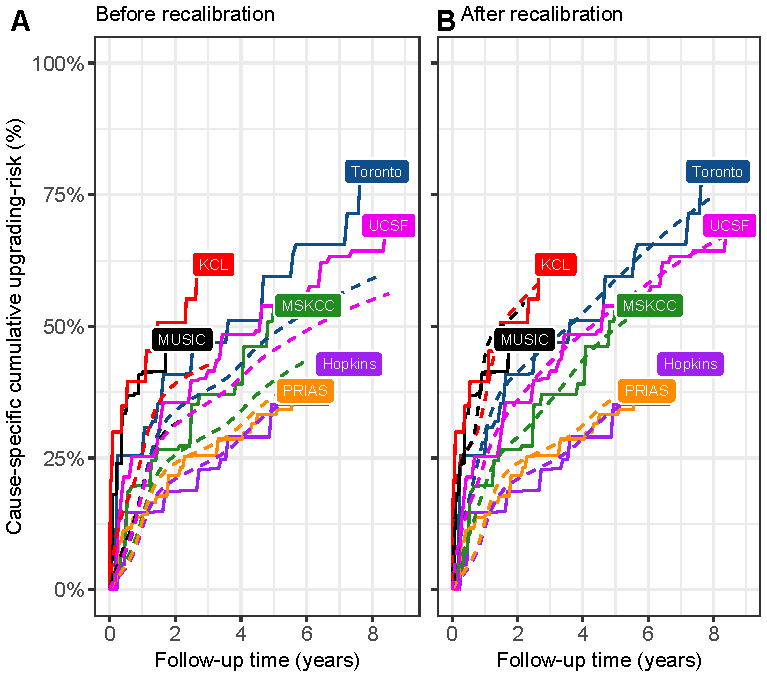
\includegraphics{contents/c5/images/c5_fig_app2.pdf}}
\caption{\textbf{Calibration-in-the-large of our model:}. In \textbf{Panel~A} we can see that our model is not well calibrated for use in KCL, MUSIC, Toronto and MSKCC. In \textbf{Panel~B} we can see that calibration of model predictions improved in KCL, MUSIC, Toronto and MSKCC cohorts after recalibrating our model. Recalibration was not necessary for Hopkins cohort. Full names of Cohorts are \textit{PRIAS}: Prostate Cancer International Active Surveillance, \textit{Toronto}: University of Toronto Active Surveillance, \textit{Hopkins}: Johns Hopkins Active Surveillance, \textit{MSKCC}: Memorial Sloan Kettering Cancer Center Active Surveillance, \textit{KCL}: King's College London Active Surveillance, \textit{MUSIC}: Michigan Urological Surgery Improvement Collaborative Active Surveillance, \textit{UCSF}: University of California San Francisco Active Surveillance.}
\label{c5:fig:calib_before_after}
\end{figure}


\textbf{\textit{Recalibrated PRIAS Model Versus Individual Joint Models For Each Cohort}}
We wanted to check if our recalibrated PRIAS model performed as good as a new joint model that could be fitted to the external cohorts. To this end, we predicted cause-specific cumulative upgrading-risk for each patient from each cohort using two sets of models, namely the recalibrated PRIAS model for each cohort, and a new joint model fitted to each cohort. The difference in predicted cause-specific cumulative upgrading-risk from these models is shown in Figure~\ref{c5:fig:calib_in_small}. We can see that the difference is smaller in those cohorts in which the effects of $\log_2 (\mbox{PSA} + 1)$ value and velocity were similar to that of PRIAS~(Table~\ref{c5:tab:PSA_survival_gap3}). For example, the Hopkins cohort had parameter estimates similar to that of PRIAS, and consequently, the difference in predicted risks for this cohort is smallest. The opposite of this phenomenon holds for the MUSIC and KCL cohorts.
 
\begin{figure}
\centerline{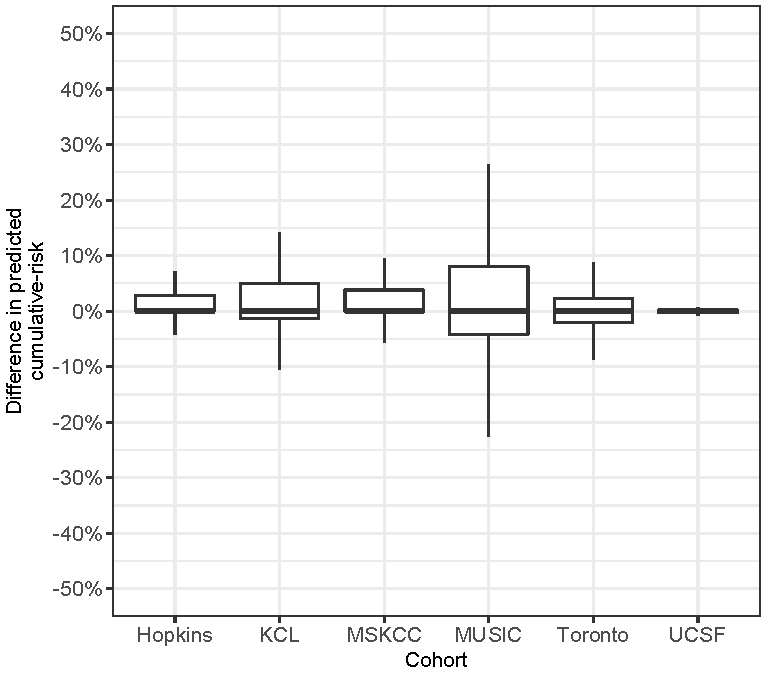
\includegraphics{contents/c5/images/c5_fig_app3.pdf}}
\caption{\textbf{Comparison of predictions from recalibrated PRIAS model with individual joint models fitted to external cohorts:} On Y-axis we show the difference between predicted cause-specific cumulative upgrading-risk for individual patients using two models, namely the recalibrated PRIAS model for each cohort, and individual joint model fitted to each cohort. The figure shows that the difference is smaller in those cohorts in which the effects of $\log_2 (\mbox{PSA} + 1)$ value and velocity were similar to that of PRIAS~(Table~\ref{c5:tab:PSA_survival_gap3}). Full names of Cohorts are \textit{PRIAS}: Prostate Cancer International Active Surveillance, \textit{Toronto}: University of Toronto Active Surveillance, \textit{Hopkins}: Johns Hopkins Active Surveillance, \textit{MSKCC}: Memorial Sloan Kettering Cancer Center Active Surveillance, \textit{KCL}: King's College London Active Surveillance, \textit{MUSIC}: Michigan Urological Surgery Improvement Collaborative Active Surveillance, \textit{UCSF}: University of California San Francisco Active Surveillance.}
\label{c5:fig:calib_in_small}
\end{figure}

\textbf{\textit{Validation of Dynamic Cumulative-Risk Predictions}}
The cumulative-risk predictions from the joint model are dynamic in nature. That is, they update as more data becomes available over time. Consequently, the discrimination and prediction error of the joint model also depend on the available data. We assessed these two measures dynamically in the PRIAS cohort (interval validation) and in the largest six external cohorts that are part of the GAP3 database. For discrimination, we utilized the time-varying area under the receiver operating characteristic curve or time-varying AUC~\citep{rizopoulos2017dynamic}. For time-varying prediction error, we assessed the mean absolute prediction error or MAPE~\citep{rizopoulos2017dynamic}. The AUC indicates how well the model discriminates between patients who experience upgrading, and those do not. The MAPE indicates how accurately the model predicts upgrading. Both AUC and MAPE are restricted to $[0,1]$. However, it is preferred that AUC $>$ 0.5 because an AUC $\leq$ 0.5 indicates that the model performs worse than random discrimination. Ideally, MAPE should be 0.

We calculate AUC and MAPE in a time-dependent manner. More specifically, given the time of latest biopsy $t$, and history of PSA measurements up to time $v$, we calculate AUC and MAPE for a medically relevant time frame $(t, v]$, within which the occurrence of upgrading is of interest. In the case of prostate cancer, at any point in time $v$, it is of interest to identify patients who may have experienced upgrading in the last one year $(v-1, v]$. That is, we set $t=v-1$. We then calculate AUC and MAPE at a gap of every six months (follow-up schedule of PRIAS). That is, $v \epsilon \{1, 1.5, \ldots \}$ years. To obtain reliable estimates of AUC and MAPE, in each cohort, we restrict $v$ to a maximum time point $v_{\mbox{max}}$, such that there are at least ten patients who experience upgrading after $v_{\mbox{max}}$. This maximum time point $v_{\mbox{max}}$ differs between cohorts, and is given in Table~\ref{c5:tab:max_pred_time}.

\begin{table}
\small
\centering
\caption{\textbf{Maximum follow-up period up to which we can reliably predict upgrading-risk and create personalized schedules}. In each cohort, this time point is chosen such that there are at least 10 patients who experience upgrading after this time point. Full names of Cohorts are \textit{PRIAS}: Prostate Cancer International Active Surveillance, \textit{Toronto}: University of Toronto Active Surveillance, \textit{Hopkins}: Johns Hopkins Active Surveillance, \textit{MSKCC}: Memorial Sloan Kettering Cancer Center Active Surveillance, \textit{KCL}: King's College London Active Surveillance, \textit{MUSIC}: Michigan Urological Surgery Improvement Collaborative Active Surveillance, \textit{UCSF}: University of California San Francisco Active Surveillance.}
\label{c5:tab:max_pred_time}
\begin{tabular}{l|r}
\hline
\hline
Cohort & \parbox[t]{3.5cm}{Maximum Prediction\\Time (years)}\\
\hline
PRIAS & 6\\
KCL & 3\\
MUSIC & 2\\
Toronto & 8\\
MSKCC & 6\\
Hopkins & 7\\
UCSF & 8.5\\
\hline
\end{tabular}    
\end{table}

The results for estimates of AUC and MAPE are summarized in Figure~\ref{c5:fig:auc_pe_recalib}, and in Table~\ref{c5:tab:AUC_PE_PRIAS} to Table~\ref{c5:tab:AUC_PE_MUSIC}. Results are based on the recalibrated PRIAS model for the GAP3 cohorts. The results show that AUC remains more or less constant in all cohorts as more data becomes available for patients. The AUC obtains a moderate value, roughly between 0.5 and 0.7 for all cohorts. On the other hand, MAPE reduces by a big margin after year one of follow-up. This could be because of two reasons. Firstly, MAPE at year one is based only on four PSA measurements gathered in the first year of follow-up, whereas after year one number of PSA measurements increases. Secondly, patients in year one consist of two sub-populations, namely patients with a correct Gleason grade group~1 at the time of inclusion in AS, and patients who probably had Gleason grade group~2 at inclusion but were misclassified by the urologist as Gleason grade group~1 patients. To remedy this problem, a biopsy for all patients at year one is commonly recommended in all AS programs~\citep{bokhorst2015compliance}.

\begin{figure}
\centerline{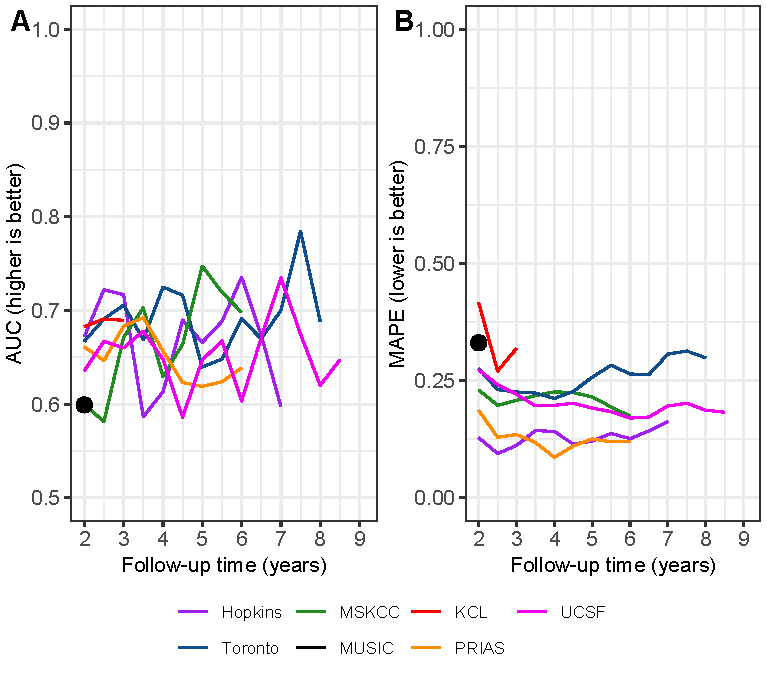
\includegraphics{contents/c5/images/c5_fig_app4.pdf}}
\caption{\textbf{Validation of dynamic predictions of cause-specific cumulative upgrading-risk}. In \textbf{Panel~A} area under the receiver operating characteristic curve or AUC (measure of discrimination) is between 0.6 and 0.7. \textbf{Panel~B} we can see that the time dependent root mean squared prediction error or MAPE is similar for PRIAS and Hopkins cohorts. The bootstrapped 95\% confidence interval for these estimates are presented in Table~\ref{c5:tab:AUC_PE_PRIAS} to Table~\ref{c5:tab:AUC_PE_KCL}. Full names of Cohorts are \textit{PRIAS}: Prostate Cancer International Active Surveillance, \textit{Toronto}: University of Toronto Active Surveillance, \textit{Hopkins}: Johns Hopkins Active Surveillance, \textit{MSKCC}: Memorial Sloan Kettering Cancer Center Active Surveillance, \textit{KCL}: King's College London Active Surveillance, \textit{MUSIC}: Michigan Urological Surgery Improvement Collaborative Active Surveillance, \textit{UCSF}: University of California San Francisco Active Surveillance.}
\label{c5:fig:auc_pe_recalib}
\end{figure}

\begin{table}
\small
\centering
\caption{\textbf{Internal validation of predictions of upgrading in PRIAS cohort}. The area under the receiver operating characteristic curve or AUC (measure of discrimination) and mean absolute prediction error or MAPE are calculated over the follow-up period at a gap of 6 months. In addition bootstrapped 95\% confidence intervals (CI) are also presented.}
\label{c5:tab:AUC_PE_PRIAS}
\begin{tabular}{r|r|r}
\hline
\hline
Follow-up period (years) & AUC (95\% CI) & MAPE (95\%CI)\\ 
\hline
1.0 to 2.0 & 0.661 [0.647, 0.678] & 0.187 [0.183, 0.191]\\
1.5 to 2.5 & 0.647 [0.596, 0.688] & 0.129 [0.122, 0.140]\\
2.0 to 3.0 & 0.683 [0.642, 0.723] & 0.135 [0.125, 0.146]\\
2.5 to 3.5 & 0.692 [0.632, 0.748] & 0.118 [0.111, 0.128]\\
3.0 to 4.0 & 0.657 [0.603, 0.709] & 0.086 [0.080, 0.092]\\
3.5 to 4.5 & 0.623 [0.582, 0.660] & 0.111 [0.105, 0.116]\\
4.0 to 5.0 & 0.619 [0.582, 0.654] & 0.126 [0.118, 0.131]\\
4.5 to 5.5 & 0.624 [0.537, 0.711] & 0.119 [0.103, 0.135]\\
5.0 to 6.0 & 0.639 [0.582, 0.696] & 0.121 [0.103, 0.138]\\
\hline
\end{tabular}    
\end{table}

\begin{table}
\small
\centering
\caption{\textbf{External validation of predictions of upgrading in University of Toronto Active Surveillance cohort}. The area under the receiver operating characteristic curve or AUC (measure of discrimination) and mean absolute prediction error or MAPE are calculated over the follow-up period at a gap of 6 months. In addition bootstrapped 95\% confidence intervals (CI) are also presented.}
\label{c5:tab:AUC_PE_Toronto}
\begin{tabular}{r|r|r}
\hline
\hline
Follow-up period (years) & AUC (95\% CI) & MAPE (95\%CI)\\ 
\hline
1.0 to 2.0 & 0.667 [0.634, 0.712] & 0.276 [0.259, 0.296]\\
1.5 to 2.5 & 0.691 [0.651, 0.730] & 0.231 [0.205, 0.254]\\
2.0 to 3.0 & 0.706 [0.637, 0.762] & 0.226 [0.196, 0.260]\\
2.5 to 3.5 & 0.669 [0.586, 0.741] & 0.224 [0.195, 0.258]\\
3.0 to 4.0 & 0.725 [0.649, 0.806] & 0.212 [0.184, 0.238]\\
3.5 to 4.5 & 0.716 [0.642, 0.793] & 0.227 [0.206, 0.258]\\
4.0 to 5.0 & 0.640 [0.579, 0.717] & 0.257 [0.222, 0.312]\\
4.5 to 5.5 & 0.648 [0.579, 0.740] & 0.283 [0.247, 0.326]\\
5.0 to 6.0 & 0.691 [0.608, 0.793] & 0.264 [0.232, 0.302]\\
5.5 to 6.5 & 0.670 [0.543, 0.776] & 0.263 [0.227, 0.307]\\
6.0 to 7.0 & 0.700 [0.544, 0.851] & 0.307 [0.258, 0.363]\\
6.5 to 7.5 & 0.785 [0.640, 0.866] & 0.313 [0.272, 0.360]\\
7.0 to 8.0 & 0.688 [0.532, 0.786] & 0.299 [0.249, 0.361]\\
\hline
\end{tabular}    
\end{table}

\begin{table}
\small
\centering
\caption{\textbf{External validation of predictions of upgrading in University of California San Francisco Active Surveillance cohort}. The area under the receiver operating characteristic curve or AUC (measure of discrimination) and mean absolute prediction error or MAPE are calculated over the follow-up period at a gap of 6 months. In addition bootstrapped 95\% confidence intervals (CI) are also presented.}
\label{c5:tab:AUC_PE_UCSF}
\begin{tabular}{r|r|r}
\hline
\hline
Follow-up period (years) & AUC (95\% CI) & MAPE (95\%CI)\\ 
\hline
1.0 to 2.0 & 0.635 [0.595, 0.677] & 0.273 [0.266, 0.281]\\
1.5 to 2.5 & 0.667 [0.628, 0.715] & 0.241 [0.224, 0.259]\\
2.0 to 3.0 & 0.660 [0.600, 0.713] & 0.221 [0.205, 0.238]\\
2.5 to 3.5 & 0.678 [0.614, 0.757] & 0.197 [0.175, 0.214]\\
3.0 to 4.0 & 0.648 [0.574, 0.707] & 0.197 [0.179, 0.221]\\
3.5 to 4.5 & 0.586 [0.525, 0.638] & 0.202 [0.180, 0.229]\\
4.0 to 5.0 & 0.647 [0.590, 0.754] & 0.192 [0.168, 0.217]\\
4.5 to 5.5 & 0.667 [0.582, 0.773] & 0.184 [0.159, 0.220]\\
5.0 to 6.0 & 0.603 [0.496, 0.696] & 0.170 [0.144, 0.207]\\
5.5 to 6.5 & 0.671 [0.576, 0.786] & 0.173 [0.145, 0.202]\\
6.0 to 7.0 & 0.735 [0.663, 0.794] & 0.196 [0.166, 0.219]\\
6.5 to 7.5 & 0.675 [0.565, 0.769] & 0.202 [0.168, 0.231]\\
7.0 to 8.0 & 0.620 [0.518, 0.740] & 0.187 [0.144, 0.217]\\
7.5 to 8.5 & 0.647 [0.538, 0.787] & 0.183 [0.146, 0.222]\\
\hline
\end{tabular}    
\end{table}

\begin{table}
\small
\centering
\caption{\textbf{External validation of predictions of upgrading in Johns Hopkins Active Surveillance cohort}. The area under the receiver operating characteristic curve or AUC (measure of discrimination) and mean absolute prediction error or MAPE are calculated over the follow-up period at a gap of 6 months. In addition bootstrapped 95\% confidence intervals (CI) are also presented.}
\label{c5:tab:AUC_PE_Hopkins}
\begin{tabular}{r|r|r}
\hline
\hline
Follow-up period (years) & AUC (95\% CI) & MAPE (95\%CI)\\ 
\hline
1.0 to 2.0 & 0.672 [0.604, 0.744] & 0.128 [0.115, 0.141]\\
1.5 to 2.5 & 0.722 [0.652, 0.792] & 0.095 [0.081, 0.111]\\
2.0 to 3.0 & 0.717 [0.638, 0.777] & 0.112 [0.100, 0.123]\\
2.5 to 3.5 & 0.587 [0.493, 0.704] & 0.144 [0.129, 0.154]\\
3.0 to 4.0 & 0.613 [0.486, 0.742] & 0.141 [0.126, 0.156]\\
3.5 to 4.5 & 0.690 [0.594, 0.783] & 0.115 [0.100, 0.133]\\
4.0 to 5.0 & 0.666 [0.572, 0.754] & 0.121 [0.104, 0.147]\\
4.5 to 5.5 & 0.688 [0.519, 0.779] & 0.137 [0.119, 0.161]\\
5.0 to 6.0 & 0.735 [0.676, 0.820] & 0.126 [0.102, 0.152]\\
5.5 to 6.5 & 0.674 [0.581, 0.765] & 0.143 [0.121, 0.172]\\
6.0 to 7.0 & 0.597 [0.472, 0.712] & 0.163 [0.126, 0.195]\\
\hline
\end{tabular}    
\end{table}

\begin{table}
\small
\centering
\caption{\textbf{External validation of predictions of upgrading in Memorial Sloan Kettering Cancer Center Active Surveillance cohort}. The area under the receiver operating characteristic curve or AUC (measure of discrimination) and mean absolute prediction error or MAPE are calculated over the follow-up period at a gap of 6 months. In addition bootstrapped 95\% confidence intervals (CI) are also presented.}
\label{c5:tab:AUC_PE_MSKCC}
\begin{tabular}{r|r|r}
\hline
\hline
Follow-up period (years) & AUC (95\% CI) & MAPE (95\%CI)\\ 
\hline
1.0 to 2.0 & 0.599 [0.518, 0.671]  & 0.230 [0.207, 0.256]\\
1.5 to 2.5 & 0.581 [0.504, 0.663]  & 0.198 [0.168, 0.235]\\
2.0 to 3.0 & 0.671 [0.599, 0.741]  & 0.208 [0.182, 0.232]\\
2.5 to 3.5 & 0.703 [0.610, 0.777]  & 0.218 [0.197, 0.246]\\
3.0 to 4.0 & 0.629 [0.499, 0.706]  & 0.226 [0.194, 0.259]\\
3.5 to 4.5 & 0.664 [0.589, 0.756]  & 0.225 [0.199, 0.262]\\
4.0 to 5.0 & 0.747 [0.642, 0.841]  & 0.215 [0.188, 0.247]\\
4.5 to 5.5 & 0.719 [0.597, 0.852]  & 0.194 [0.165, 0.232]\\
5.0 to 6.0 & 0.698 [0.565, 0.792]  & 0.174 [0.136, 0.227]\\
\hline
\end{tabular}    
\end{table}

\begin{table}
\small
\centering
\caption{\textbf{External validation of predictions of upgrading in King's College London Active Surveillance cohort}. The area under the receiver operating characteristic curve or AUC (measure of discrimination) and mean absolute prediction error or MAPE are calculated over the follow-up period at a gap of 6 months. In addition bootstrapped 95\% confidence intervals (CI) are also presented.}
\label{c5:tab:AUC_PE_KCL}
\begin{tabular}{r|r|r}
\hline
\hline
Follow-up period (years) & AUC (95\% CI) & MAPE (95\%CI)\\ 
\hline
1.0 to 2.0 & 0.683 [0.604, 0.753] & 0.416 [0.396, 0.445] \\
1.5 to 2.5 & 0.691 [0.621, 0.766] & 0.271 [0.246, 0.297] \\
2.0 to 3.0 & 0.689 [0.616, 0.785] & 0.319 [0.282, 0.344] \\
\hline
\end{tabular}    
\end{table}

\begin{table}
\small
\centering
\caption{\textbf{External validation of predictions of upgrading in Michigan Urological Surgery Improvement Collaborative Active Surveillance cohort}. The area under the receiver operating characteristic curve or AUC (measure of discrimination) and mean absolute prediction error or MAPE are calculated over the follow-up period at a gap of 6 months. In addition bootstrapped 95\% confidence intervals (CI) are also presented.}
\label{c5:tab:AUC_PE_MUSIC}
\begin{tabular}{r|r|r}
\hline
\hline
Follow-up period (years) & AUC (95\% CI) & MAPE (95\%CI)\\ 
\hline
1.0 to 2.0 & 0.599 [0.553, 0.632] & 0.331 [0.317, 0.348]\\
\hline
\end{tabular}    
\end{table}

\section{Source Code}
\label{c5:appendix:source_code}
The R code for fitting the joint model to the PRIAS dataset, is at \url{https://github.com/anirudhtomer/prias/tree/master/src/clinical_gap3}. We refer to this location as `R\_HOME' in the rest of this document. The PRIAS dataset is not openly accessible. However, access to the database can be requested via the contact links at \url{https://www.prias-project.org}.

The PRIAS dataset is in the so-called wide format and also requires the removal of incorrect entries. This can be done via the R script \url{R_HOME/dataset_cleaning.R}. This will lead to two R objects, namely `prias\_final.id' and `prias\_long\_final'. The `prias\_final.id' object contains information about the time of upgrading for PRIAS patients. The `prias\_long\_final' object contains longitudinal PSA measurements, the time of biopsies and results of biopsies.

We use a joint model for time-to-event and longitudinal data to model the evolution of PSA measurements over time, and to simultaneously model their association with the risk of upgrading. The R package we use for this purpose is called \textbf{JMbayes} (https://cran.r-project.org/web/packages/JMbayes/JMbayes.pdf). The API we use, however, is currently not hosted on CRAN, and can be found here:
\url{https://github.com/anirudhtomer/JMbayes}. The joint model can be fitted via the script \url{R_HOME/analysis.R}. It takes roughly 6 hours to run on an Intel Core-i5 machine with four cores and 8GB of RAM. 

The graphs presented in the main manuscript, and the appendix can be generated by the scripts in \url{R_HOME/plots/}.

Validations can be done using the scripts \url{R_HOME/validation/auc_brier/auc_calculator.R}, and \url{R_HOME/validation/auc_brier/gof_calculator.R}. For external validation access to GAP3 database is required.

Once a joint model is fitted to the PRIAS dataset, personalized schedules of biopsies based on the risk of upgrading for new patients can be developed as shown in the script \url{R_HOME/plots/demo_schedule_supplementary.R} or directly using the script \url{https://raw.githubusercontent.com/anirudhtomer/prias/master/src/lastpaper/pers_schedule_api.R}.

Source code for the shiny web application which provides biopsy schedules for patients can be found at \url{R_HOME/shinyapp}
\end{subappendices}

\clearpage
\bibliographystyle{apalike}
\bibliography{c5_bib}